\section{Tunable Couplers}
\label{sec:tunable_couplers}

Qubits in our device are coupled through tunable couplers.
They allow us to mediate interaction between the qubits and perform two-qubits gates.
They are composed of two planar waveguide, one of them with a fixed coupling term $J_{\text{fixed}}$.
The other is instead flux tunable, meaning that its coupling term $J_{\text{tunable}}(\Phi)$ can be tuned with the magnetic flux generated by a flux line and going into a SQUID loop placed on the waveguide as depicted in \cref{fig:tun_coupl}.

\begin{figure}
    \centering
    

\tikzset{every picture/.style={line width=0.75pt}} %set default line width to 0.75pt        

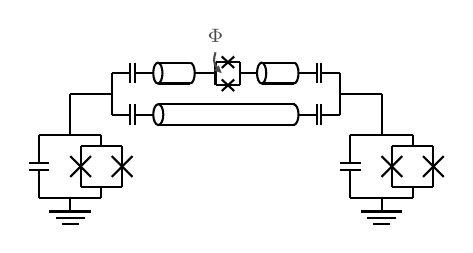
\begin{tikzpicture}[x=0.75pt,y=0.75pt,yscale=-1,xscale=1]
%uncomment if require: \path (0,300); %set diagram left start at 0, and has height of 300

%Straight Lines [id:da07218492708859259] 
\draw    (165,140) -- (135,140) ;
%Shape: Capacitor [id:dp26518043172092054] 
\draw   (135,140) -- (135,153.5) (140,156.5) -- (130,156.5) (140,153.5) -- (130,153.5) (135,156.5) -- (135,170) ;
%Straight Lines [id:da13302415031214743] 
\draw    (135,170) -- (165,170) ;
%Straight Lines [id:da17130629114618245] 
\draw    (155,145) -- (175,145) ;
%Straight Lines [id:da29260280538604033] 
\draw    (155,165) -- (175,165) ;
%Straight Lines [id:da49230231307780326] 
\draw    (175,145) -- (175,165) ;
%Straight Lines [id:da3653947605727903] 
\draw    (155,145) -- (155,165) ;
%Straight Lines [id:da44803766219329755] 
\draw    (165,140) -- (165,145) ;
%Straight Lines [id:da9101556277746032] 
\draw    (165,165) -- (165,170) ;
%Straight Lines [id:da006475878830819681] 
\draw    (170,150) -- (180,160) ;
%Straight Lines [id:da33120831736226397] 
\draw    (150,150) -- (160,160) ;
%Straight Lines [id:da11004761294731558] 
\draw    (160,150) -- (150,160) ;
%Straight Lines [id:da9445264009597942] 
\draw    (180,150) -- (170,160) ;
%Shape: Ground [id:dp22167919288849824] 
\draw   (140, 176.67) -- (160, 176.67) ;
\draw   (143, 179.67) -- (157, 179.67) ;
\draw   (146, 182.67) -- (154, 182.67) ;
\draw   (150, 170) -- (150, 176.67) ;
%Straight Lines [id:da42940827257352] 
\draw    (315,140) -- (285,140) ;
%Shape: Capacitor [id:dp49877304955829627] 
\draw   (285,140) -- (285,153.5) (290,156.5) -- (280,156.5) (290,153.5) -- (280,153.5) (285,156.5) -- (285,170) ;
%Straight Lines [id:da7324100328789034] 
\draw    (285,170) -- (315,170) ;
%Straight Lines [id:da208048098521316] 
\draw    (305,145) -- (325,145) ;
%Straight Lines [id:da8572518030578566] 
\draw    (305,165) -- (325,165) ;
%Straight Lines [id:da5742858039200953] 
\draw    (325,145) -- (325,165) ;
%Straight Lines [id:da3966431831849069] 
\draw    (305,145) -- (305,165) ;
%Straight Lines [id:da19183525795672862] 
\draw    (315,140) -- (315,145) ;
%Straight Lines [id:da004743615923411104] 
\draw    (315,165) -- (315,170) ;
%Straight Lines [id:da17738152912719607] 
\draw    (320,150) -- (330,160) ;
%Straight Lines [id:da8678835567326026] 
\draw    (300,150) -- (310,160) ;
%Straight Lines [id:da28374358820735224] 
\draw    (310,150) -- (300,160) ;
%Straight Lines [id:da24817307713778236] 
\draw    (330,150) -- (320,160) ;
%Shape: Ground [id:dp861700376356459] 
\draw   (290, 176.67) -- (310, 176.67) ;
\draw   (293, 179.67) -- (307, 179.67) ;
\draw   (296, 182.67) -- (304, 182.67) ;
\draw   (300, 170) -- (300, 176.67) ;
%Straight Lines [id:da6625685419222695] 
\draw    (150,140) -- (150,120) ;
%Straight Lines [id:da2635718281625268] 
\draw    (300,140) -- (300,120) ;
%Straight Lines [id:da3980890926472094] 
\draw    (170,120) -- (150,120) ;
%Straight Lines [id:da6516978234304753] 
\draw    (170,120) -- (170,110) ;
%Straight Lines [id:da8682527218489697] 
\draw    (170,130) -- (170,120) ;
%Shape: Capacitor [id:dp26464751353501326] 
\draw   (170,110) -- (179,110) (181,105) -- (181,115) (179,105) -- (179,115) (181,110) -- (190,110) ;
%Shape: Capacitor [id:dp9673816527519772] 
\draw   (170,130) -- (179,130) (181,125) -- (181,135) (179,125) -- (179,135) (181,130) -- (190,130) ;
%Shape: Ellipse [id:dp26511497109868176] 
\draw   (190,110) .. controls (190,107.24) and (191,105) .. (192.22,105) .. controls (193.45,105) and (194.45,107.24) .. (194.45,110) .. controls (194.45,112.76) and (193.45,115) .. (192.22,115) .. controls (191,115) and (190,112.76) .. (190,110) -- cycle ;
%Straight Lines [id:da14470289747688758] 
\draw    (192.22,105) -- (207.79,105) ;
%Straight Lines [id:da773223714503521] 
\draw    (192.22,115) -- (207.79,115) ;
%Shape: Arc [id:dp18440292021788673] 
\draw  [draw opacity=0] (207.79,105) .. controls (209.01,105.02) and (210,107.25) .. (210,110) .. controls (210,112.75) and (209.01,114.98) .. (207.79,115) -- (207.78,110) -- cycle ; \draw   (207.79,105) .. controls (209.01,105.02) and (210,107.25) .. (210,110) .. controls (210,112.75) and (209.01,114.98) .. (207.79,115) ;  

%Shape: Ellipse [id:dp6247106434937635] 
\draw   (190,130) .. controls (190,127.24) and (191.09,125) .. (192.43,125) .. controls (193.77,125) and (194.86,127.24) .. (194.86,130) .. controls (194.86,132.76) and (193.77,135) .. (192.43,135) .. controls (191.09,135) and (190,132.76) .. (190,130) -- cycle ;
%Straight Lines [id:da5902234364980534] 
\draw    (192.43,125) -- (258.06,125) ;
%Straight Lines [id:da6759349880739789] 
\draw    (192.43,135) -- (258.06,135) ;
%Shape: Arc [id:dp6456040885907672] 
\draw  [draw opacity=0] (257.59,125) .. controls (258.92,125.02) and (260,127.25) .. (260,130) .. controls (260,132.75) and (258.92,134.98) .. (257.59,135) -- (257.57,130) -- cycle ; \draw   (257.59,125) .. controls (258.92,125.02) and (260,127.25) .. (260,130) .. controls (260,132.75) and (258.92,134.98) .. (257.59,135) ;  

%Shape: Ellipse [id:dp7275157055864581] 
\draw   (240,110) .. controls (240,107.24) and (241,105) .. (242.22,105) .. controls (243.45,105) and (244.45,107.24) .. (244.45,110) .. controls (244.45,112.76) and (243.45,115) .. (242.22,115) .. controls (241,115) and (240,112.76) .. (240,110) -- cycle ;
%Straight Lines [id:da6315731480773339] 
\draw    (242.22,105) -- (257.79,105) ;
%Straight Lines [id:da6406460700415237] 
\draw    (242.22,115) -- (257.79,115) ;
%Shape: Arc [id:dp38475017613626794] 
\draw  [draw opacity=0] (257.79,105) .. controls (259.01,105.02) and (260,107.25) .. (260,110) .. controls (260,112.75) and (259.01,114.98) .. (257.79,115) -- (257.78,110) -- cycle ; \draw   (257.79,105) .. controls (259.01,105.02) and (260,107.25) .. (260,110) .. controls (260,112.75) and (259.01,114.98) .. (257.79,115) ;  

%Straight Lines [id:da060781913550373545] 
\draw    (210,110) -- (220,110) ;
%Straight Lines [id:da15398066157627577] 
\draw    (232,104.77) -- (232,115.85) ;
%Straight Lines [id:da14222494293706922] 
\draw    (220,104.77) -- (220,115.85) ;
%Straight Lines [id:da6561755710145185] 
\draw    (232,115.85) -- (220,115.85) ;
%Straight Lines [id:da742586164519965] 
\draw    (232,104.77) -- (220,104.77) ;
%Straight Lines [id:da21146645385961227] 
\draw    (229,113.08) -- (223,118.63) ;
%Straight Lines [id:da3871753118676642] 
\draw    (229,102) -- (223,107.54) ;
%Straight Lines [id:da5637422527324993] 
\draw    (229,107.54) -- (223,102) ;
%Straight Lines [id:da9093097576487559] 
\draw    (229,118.63) -- (223,113.08) ;

%Straight Lines [id:da4289728577327423] 
\draw    (232,110) -- (240,110) ;
%Shape: Capacitor [id:dp8421236410162245] 
\draw   (260,110) -- (269,110) (271,105) -- (271,115) (269,105) -- (269,115) (271,110) -- (280,110) ;
%Straight Lines [id:da787480793091047] 
\draw    (280,120) -- (280,110) ;
%Straight Lines [id:da5372127440829679] 
\draw    (280,130) -- (280,120) ;
%Shape: Capacitor [id:dp09893187150822791] 
\draw   (260,130) -- (269,130) (271,125) -- (271,135) (269,125) -- (269,135) (271,130) -- (280,130) ;
%Straight Lines [id:da43455598058651357] 
\draw    (300,120) -- (280,120) ;
%Curve Lines [id:da7527622826730622] 
\draw [color={rgb, 255:red, 74; green, 74; blue, 74 }  ,draw opacity=1 ]   (220,100) .. controls (219.34,102.74) and (218.4,104.58) .. (220.96,107.82) ;
\draw [shift={(223,110)}, rotate = 223.23] [fill={rgb, 255:red, 74; green, 74; blue, 74 }  ,fill opacity=1 ][line width=0.08]  [draw opacity=0] (3.57,-1.72) -- (0,0) -- (3.57,1.72) -- cycle    ;

% Text Node
\draw (220,97) node [anchor=south] [inner sep=0.75pt]  [font=\scriptsize,color={rgb, 255:red, 74; green, 74; blue, 74 }  ,opacity=1 ] [align=left] {$\displaystyle \Phi $};


\end{tikzpicture}
    \vspace{-1cm}
    \caption{Schematic representation of two qubits connected by a tunable coupler}
    \label{fig:tun_coupl}
\end{figure}

The SQUID loop connected to the coupler allows us to control the interaction between the two qubits.
To minimise the interaction between the two qubits and the ZZ crosstalk, the DC flux driving the SQUID loop has to be calibrated to the operation point.

To implement a two-qubit gate, a sinusoidal pulse is sent on top of the DC flux to the SQUID loop.
If the modulation frequency of this pulse matches a transition of the two-qubit system, it will perform a two-qubit gate.
In this way we are able to turn on interactions between specific levels of the qubits.
\textcolor{red}{Reference the next section maybe.}
